\section{系统评估}
\label{kvdirect:sec:eval}
\label{kvdirect:sec:evaluation}
\label{kvdirect:sec:system-benchmark}

\subsection{系统实现}

为了提高开发效率,使用英特尔FPGA SDK for OpenCL~ \cite {aoc}来合成OpenCL的硬件逻辑。
键值处理器采用1.1万行OpenCL代码实现,所有内核都完全流水线化,即吞吐量是每个时钟周期一次操作。
凭借180~MHz的时钟频率,可以在180~M op/s下处理键值操作,如果网络,DRAM或PCIe不是瓶颈。


%\textbf{网络协议,客户端}


\subsection{测试床与评估方法}

本节在8台服务器和1台Arista DCS-7060CX-32S交换机的测试台上评估KV-Direct。
每台服务器配备两个禁用超线程的8核Xeon E5-2650 v2 CPU,形成两个通过QPI Link连接的NUMA节点。每个NUMA节点都装有8个DIMM 8~GiB三星DDR3-1333 ECC RAM,每台服务器上总共有128~GiB的主机内存。
可编程网卡~ \cite {caulfield2016cloud}连接到CPU 0的PCIe root complex,其40~Gbps以太网端口连接到交换机。可编程网卡在分叉的Gen3 x16物理连接器中有两个PCIe Gen3 x8链路。
经过测试的服务器配备SuperMicro X9DRG-QF主板和一个运行Archlinux的120~GB SATA SSD(内核版本4.11.9-1)。

对于系统基准测试,使用YCSB工作负载 \cite {cooper2010benchmarking}。
对于偏斜(skewed)的Zipf工作负载,本文选择偏差(skewness)0.99并将其称为\textit {长尾}工作负载。

在每个基准测试之前,根据键值大小,访问模式和目标内存利用率来调整哈希索引比率,内联阈值和负载分派比率。
然后生成具有给定大小的随机键值对。
给定内联键值大小的键大小与KV-Direct的性能无关,因为在处理期间将键填充到最长的内联键值大小。
为了测试内联案例,使用键值大小作为插槽大小的倍数(当大小为$ \leq $ 50时,即10个插槽)。为了测试非内联的情况,使用的键值大小是2减2字节的幂(对于元数据)。
作为准备的最后一步,发出PUT操作以将键值对插入空闲键值存储,直到50%内存利用率。
其他内存利用率下的性能可以从图 \ref {kvdirect:fig:mem-access-tput}中获得。

在基准测试期间,在同一个ToR中使用基于FPGA的数据包生成器 \cite {li2016clicknp}来生成批量键值操作,将它们发送到键值服务器,接收完成并测量可持续的吞吐量和延迟。
分组生成器的处理延迟通过直接环回预先校准,并从延迟测量中移除。
误差线表示$ 5^{th} $和$ 95^{th} $百分位数。

\subsection{吞吐量}

图 \ref {kvdirect:fig:ycsb-tput} 显示了YCSB均匀和长尾(偏斜Zipf)工作负载下KV-Direct的吞吐量。
三个因素可能是KV-Direct的瓶颈:时钟频率,网络和PCIe / DRAM。
对于在哈希索引中内联的5B至15B 键值,大多数GET需要一个PCIe / DRAM访问,而PUT需要两个PCIe / DRAM访问。
这种小型键值在许多系统中很普遍。在PageRank中,边的键值大小为8B。在稀疏逻辑回归中,键值大小通常为8B-16B。对于分布式系统中的顺控程序和锁,键值大小为8B。


\begin{figure}[htbp]
	\centering
	\subfloat[均匀分布。\label{kvdirect:fig:ycsb-tput-uniform}]
	{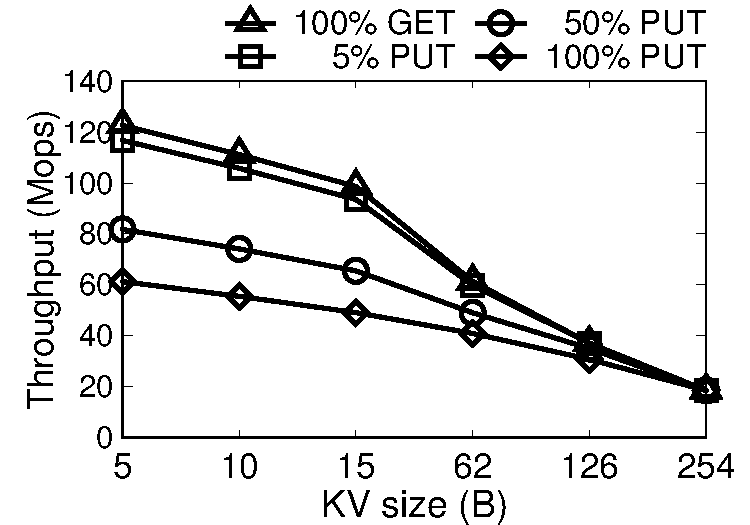
\includegraphics[width=.5\textwidth,page=1]{ycsb-tput-uniform.pdf}}
	\subfloat[长尾分布。\label{kvdirect:fig:ycsb-tput-longtail}]
	{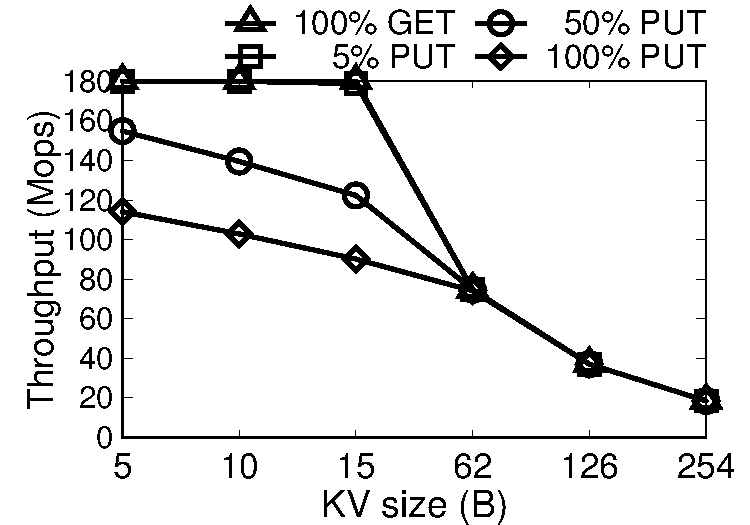
\includegraphics[width=.5\textwidth,page=1]{ycsb-tput-longtail.pdf}}
	\caption{KV-Direct 在 YCSB 负载下的吞吐量。}
	\label{kvdirect:fig:ycsb-tput}
\end{figure}


在相同的内存利用率下,由于哈希冲突的概率较高,较大的内联键值具有较低的吞吐量。
62B和更大的键值没有内联,因此它们需要额外的内存访问。
长尾工作负载比统一工作负载具有更高的吞吐量,并且能够在读密集工作负载下达到180~Mops的时钟频率范围,或达到$ \geq $ 62B 键值大小的网络吞吐量。
在长尾工作负载下,无序执行引擎在最流行的键上合并到大约15%的操作,并且板载DRAM在60%负载分配比率下具有大约60%的高速缓存命中率,这可以统一导致高达2倍的吞吐量作为统一的工作量。
如表 \ref {kvdirect:tab:kvs-compare} 所示,KV-Direct 网卡的吞吐量与具有数十个CPU核心的最先进的键值存储服务器相当。


\begin{sidewaystable}[htbp]
	\centering
	\caption{KV-Direct 与其他键值存储系统在长尾(倾斜  Zipf)负载和 10 字节小键下的比较。对于相关工作未报告的性能数字,本文使用相似的硬件来模拟这些系统,并报告粗略的测量结果。对于 CPU 绕过的系统,括号内的数字报告峰值负载和空闲情况下的功耗差异。}
	\label{kvdirect:tab:kvs-compare}
	\small
	\begin{tabular}{|l|l|l|r|r|r|r|r|r|r|}
		\toprule
		键值存储  & 注释 & 性能瓶颈 & \multicolumn{2}{c|}{吞吐量 (Mops)} & \multicolumn{2}{c|}{功耗效率 (Kops/W)} & \multicolumn{2}{c|}{平均延迟 ($\mu$s)} \\
		\cline{4-9}表 \ref {clicknp:tab:elements} 
		& & & GET & PUT & GET & PUT & GET & PUT \\
		\midrule
		Memcached~\cite{fitzpatrick2004distributed} & 传统 & CPU 核间同步 & 1.5 & 1.5 & \approx5 & \approx5 & \approx50 & \approx50 \\
		MemC3~\cite{fan2013memc3} & 传统 & 操作系统网络协议栈 & 4.3 & 4.3 & \approx14 & \approx14 & \approx50 & \approx50 \\
		RAMCloud~\cite{ousterhout2015ramcloud} & 内核绕过 & 分派线程 & 6 & 1 & \approx20 & \approx3.3 & 5 & 14 \\
		MICA~\cite{lim2014mica} & 内核绕过,24 个核,12 个网卡口 & CPU 键值处理 & 137 & 135 & 342 & 337 & 81 & 81 \\
		FaRM~\cite{dragojevic2014farm} & 单边 RDMA GET & RDMA 网卡 & 6 & 3 & \approx30 (261) & \approx15 & 4.5 & \approx10 \\
		DrTM-KV~\cite{wei2015fast} & 单边 RDMA 和 HTM & RDMA 网卡 & 115.2 & 14.3 & \approx500 (3972) & \approx60 & 3.4 & 6.3 \\
		HERD'16~\cite{kalia2016design} & 双边 RDMA, 12 核 & PCIe & 98.3 & \approx60 & \approx490 & \approx300 & 5 & 5 \\
		Xilinx'13~\cite{blott13hotcloud} & FPGA & 网络 & 13 & 13 & 106 & 106 & 3.5 & 4.5 \\
		Mega-KV~\cite{zhang2015mega} & GPU (4~GiB 板上 RAM) & GPU 键值处理 & 166 & 80 & \approx330 & \approx160 & 280 & 280 \\
		\midrule
		\textbf{KV-Direct (1 网卡)} & 可编程网卡,两个 Gen3 x8 & PCIe \& DRAM & 180 & 114 & 1487 (5454) & 942 (3454) & 4.3 & 5.4 \\
		\textbf{KV-Direct (10 网卡)} & 可编程网卡,每卡一个 Gen3 x8 & PCIe \& DRAM & 1220 & 610 & 3417 (4518) & 1708 (2259) & 4.3 & 5.4 \\
		\bottomrule
	\end{tabular}
\end{sidewaystable}


\subsection{能耗效率}

插入KV-Direct 网卡可为空闲服务器增加10.6 W的功率。
当KV-Direct服务器处于峰值吞吐量时,系统功率为121.4瓦(在墙上测量)。
与表 \ref {kvdirect:tab:kvs-compare} 中最先进的键值存储系统相比,KV-Direct的功率效率是其他系统的3倍,是第一个达到100万的通用键值存储系统 商用服务器上每瓦特的键值操作。

当拔出KV-Direct网卡时,空闲服务器的功耗为87.0瓦,因此可编程网卡,PCIe,主机内存和CPU上的守护进程的总功耗仅为34瓦。
测量的功率差异是合理的,因为CPU几乎处于空闲状态,服务器可以在KV-Direct运行时运行其他工作负载(对单侧RDMA使用相同的标准,如表 \ref{kvdirect:tab:kvs-compare} 的括号中所示)。
在这方面,KV-Direct的功率效率是基于CPU的系统的10倍。

\subsection{延迟}

图 \ref {kvdirect:fig:ycsb-lat} 显示了YCSB工作负载峰值吞吐量下KV-Direct的延迟。
在没有网络批处理的情况下,尾部延迟范围为3至9 $\mu$s,具体取决于键值大小,操作类型和键分配。
由于额外的内存访问,PUT具有比GET更高的延迟。
由于更有可能在板载DRAM中进行缓存,因此倾斜的工作负载具有比均匀更低的延迟。
由于额外的网络和PCIe传输延迟,较大的键值具有较高的延迟。
网络批处理比非批处理操作增加了不到1~$\mu$s 的延迟,但显著提高了吞吐量,已在图 \ref {kvdirect:fig:eval-network-batching} 中进行了评估。

\begin{figure}[htbp]
	\centering
	\subfloat[有批量操作。\label{kvdirect:fig:ycsb-lat-batch}]
	{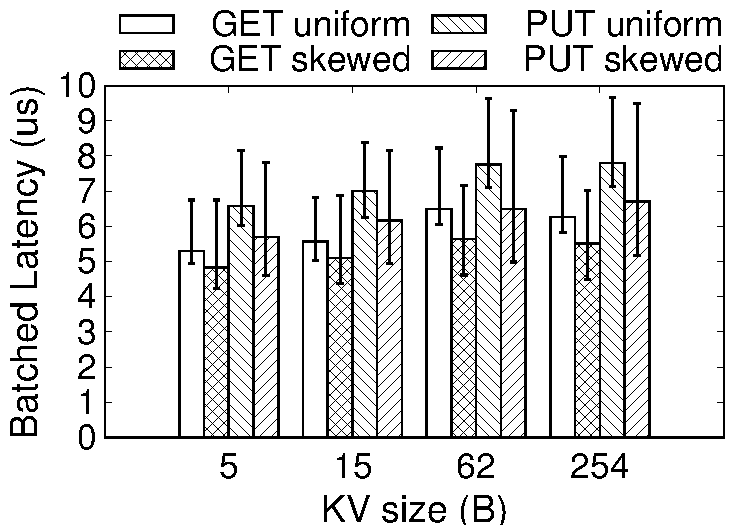
\includegraphics[width=.5\textwidth,page=1]{lat-batch.pdf}}
	\subfloat[无批量操作。\label{kvdirect:fig:ycsb-lat-nobatch}]
	{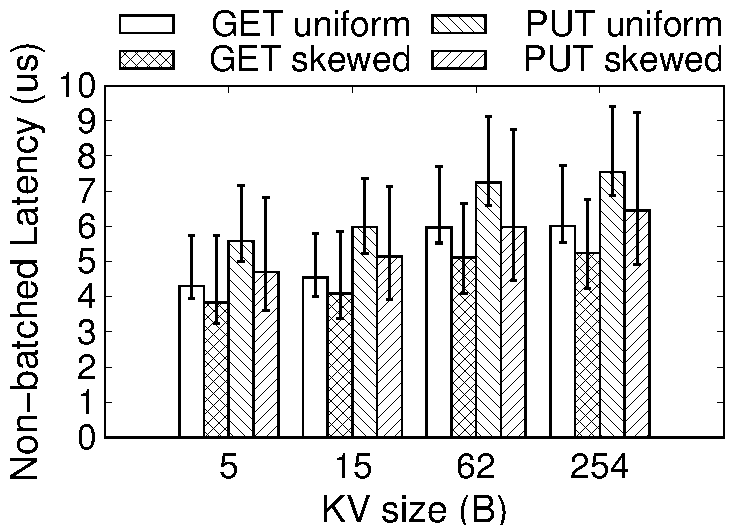
\includegraphics[width=.5\textwidth,page=1]{lat-nonbatch.pdf}}
	\caption{在YCSB工作负载的峰值吞吐量下KV-Direct的延迟。}
	\label{kvdirect:fig:ycsb-lat}
\end{figure}

\subsection{对 CPU 性能的影响}


KV-Direct旨在绕过服务器CPU,仅使用一部分主机内存用于键值存储。 因此,CPU仍然可以运行其他应用程序。
当单个网卡 KV-Direct处于峰值负载时,测量对服务器上的其他工作负载的影响最小。
表 \ref {kvdirect:tab:cpu-impact} 量化了KV-Direct峰值吞吐量的影响。
除了CPU 0的顺序吞吐量以访问其自己的NUMA内存(以粗体标记的行)之外,CPU内存访问的延迟和吞吐量大多不受影响。
这是因为8个主机存储器通道可以提供比所有CPU核心消耗的更高的随机访问吞吐量,而CPU确实可以强调DRAM通道的顺序吞吐量。
当键值大小的分布相对稳定时,主机守护程序进程的影响是最小的,因为仅当不同板大小的可用槽的数量不平衡时才调用垃圾收集器。

\begin{table}[htbp]
	\centering
	\caption{当KV-Direct达到峰值吞吐量时,对CPU内存访问性能的影响。 使用英特尔性能计数器监视器(Intel PCM)V2.11测量。}
	\label{kvdirect:tab:cpu-impact}
	\small
		\begin{tabular}{l|l|r|r}
			\toprule
			\multicolumn{2}{r}{KV-Direct 状态 $\rightarrow$} & 空闲 & 繁忙 \\
			\midrule
			\multirow{4}{*}{\specialcell{随机访问延迟}} & CPU0-0 & 82.2 ns & 83.5 ns \\
            					  & CPU0-1 & 129.3 ns & 129.9 ns \\
                                  & CPU1-0 & 122.3 ns & 122.2 ns \\
                                  & CPU1-1 & 84.2 ns & 84.3 ns \\
			\midrule
            \multirow{4}{*}{\specialcell{顺序访问吞吐量}} & \textbf{CPU0-0} & \textbf{60.3 GB/s} & \textbf{55.8 GB/s} \\
            					  & CPU0-1 & 25.7 GB/s & 25.6 GB/s \\
                                  & CPU1-0 & 25.5 GB/s & 25.9 GB/s \\
                                  & CPU1-1 & 60.2 GB/s & 60.3 GB/s \\
			\midrule
			\multirow{4}{*}{\specialcell{随机访问吞吐量}} & 32B 读 & 10.53 GB/s & 10.46 GB/s \\
            						& 64B 读 & 14.41 GB/s & 14.42 GB/s \\
                                    & 32B 写 & 9.01 GB/s & 9.04 GB/s \\
                                    & 64B 写 & 12.96 GB/s & 12.94 GB/s \\
			\bottomrule
		\end{tabular}      
\end{table}

